\section{Allgemeine Änderungen}

\subsection{Organisatorisches}
\subsubsection{Struktur der Repositories}
Das ursprüngliche Projekt bestand aus zwei Teilen: der Android App, als
Client, und einem Java Backend, welches den Bot beinhaltete und die Server
Rolle einnahm. Das Versionsmanagement beider wurde bisher in einem gemeinsamen
Repository gehandhabt. Dies brachte eine gewisse Unübersichtlichkeit
mit sich. Daher haben wir für jedes Teilprojekt ein eigenes Repository angelegt.
Die Aufteilung zwischen der App und dem Backend wurde beibehalten, es kam
lediglich noch ein Teil hinzu, welchen die Service-API-Library ausfüllt. Damit
ist die aktuelle Aufteilung auf Github wie folgt:\\\\
\begin{small}
\begin{tabular}{ l l }
Altes Repository unserer Vorgänger: & https://github.com/TeamChatbot/chatbot\\
Aktuelle Android App: & https://github.com/TeamChatbot/Hablame-Android-App\\
Aktuelle Service-API-Library: &
https://github.com/TeamChatbot/hablame-service-api\\
Aktuelles Service-Botbackend: &
https://github.com/TeamChatbot/Hablame-BotBackend\\
\end{tabular}
\end{small}\\\\
Durch diese Aufteilung kann besser und unabhängiger an den einzelnen Teilprojekten gearbeitet werden.

\subsubsection{Aktuelle Aufgabenverteilung auf die Teilprojekte}
Durch das Hinzufügen der Service-API-Library ergibt sich nachfolgend
dargestellter Gesamtaufbau, bei welchem jedes Teilprojekt eine
Teilaufgabe des Gesamtsystems übernimmt:
\begin{figure}[h]
	\centering
	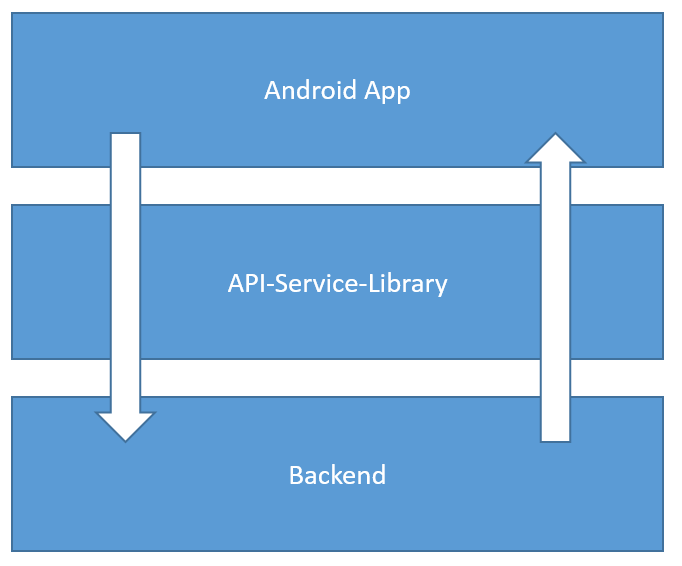
\includegraphics[width=0.7\linewidth]{ks/graphics/arch.png}
	\caption{Gesamtaufbau Hablame}
	\label{fig:arch}
\end{figure}
\\\\
Android App:
\begin{itemize}\itemsep0pt
	\item Umwandlung gesprochener Sprache in Text ("`Speech-To-Text"')
	\item Umwandlung von Text in gesprochene Sprache ("`Text-To-Speech"')
	\item Weiterleiten der Informationen mittels der API-Service-Library an das Backend
\end{itemize}
API-Service-Library:
\begin{itemize}\itemsep0pt
	\item Erstellen der Anfragen an das Backend
	\item Weitergabe der Backend-Antworten an das aufrufende System
\end{itemize}
Backend:
\begin{itemize}\itemsep0pt
	\item Hosting und Konfiguration des Chatbots
	\item Auswerten der Serviceanfragen
\end{itemize}

\subsection{Dokumentation und Projektmanagement}
	Eine Dokumentation stellt einerseits die Übersichtlichkeit und
	Nachvollziehbarkeit für Dritte und den Entwickler selbst her und verkürzt
	andererseits die Einarbeitungszeit nachfolgender Projektteams enorm. Mit
	vorhandenem Projektmanagement Tools kann die Kollaboration im Team noch weiter
	optimiert werden. Diese Ziele wurden in Form von zwei erwähnenswerten Punkten
	angestrebt, welche in den nachfolgenden Unterkapiteln erläutert werden sollen.
	
	\subsubsection{Javadocs und Codedokumentation}
		In jedem der drei Teilprojekte wurde Wert auf dokumentierten Code gelegt. Dies
		bedeutet, dass jede implementierte Klasse mitsamt jeder dort realisierten
		Methode dokumentiert ist. Das ermöglicht beim Aufruf einer Klasse bzw. Methode
		eine Anzeige dieser Javadocs, was automatisch über die IDE realisiert wird.
		Wenn beispielsweise eine neue Extension für den Chatbot realisiert werden
		soll, kann der Entwickler über die Nutzung von bereits vorhandenen
		Erweiterungen und vor allem deren dokumentierten Text nachvollziehen wie dies
		umzusetzen ist. Zusätzlich wurden Dokumentationsseiten der JavaDocs angelegt
		und im jeweiligen Repository auf Github gespeichert.
		
	\subsubsection{Redmine}
		Als einzige bekannte und weit verbreitete Projektmanagement Software, die
		quelloffen und für den eigenen Gebraucht selbst aufgesetzt werden kann, kam
		Redmine in Frage, welche auf dem für das Projekt verfügbaren Windows 2008 R2
		Server installiert und unter dem bestehenden Apache Webserver konfiguriert
		wurde. Diese ermöglicht es dem Projektteam über diverse Features effizient
		an diesem und auch künftigen Projekten zu arbeiten. Redmine enthält
		beispielsweise ein Ticketsystem, welches für Aufgabenverteilung und
		Zeitmanagement genutzt werden kann. Außerdem ist es dem Projektleiter
		möglich, auf einfache Weise einzusehen, wie der Stand einzelner Aufgaben
		ist. Ein internes Wiki\footnote{Projekt Wiki in Redmine:
		http://194.95.221.229/redmine/projects/hablame/wiki/} enthält wichtige
		Dokumentation über sensible Zugänge und Informationen, sowie Dokumente. Ein
		Kalender pro Projekt und eine E-Mail Funktion erhöht die
		Kommunikationsfähigkeit und steigert die Effizienz weiter. Über all diesen
		Möglichkeit steht natürlich die Zugriffssicherheit, welche ein integriertes
		Benutzermanagement darstellt, über welches neue Teammitglieder eingepflegt
		werden können und obsolete als inaktiv markiert, bzw. gelöscht werden können.
		Die Redmine Instanz ist über folgenden Link zu erreichen:
		http://194.95.221.229/redmine.

\subsection{Unit Testing}
	Neu ist auch das, bisher nicht beachtete, automatisierte Testen des
	Programmcodes. Hierfür wird auf das Java Framework JUnit
	zurückgegriffen.\footnote{Projektseite von JUnit: http://junit.org/} Durch das
	Nutzen eines solchen Frameworks ist es möglich automatisiert Programmcode auf
	die korrekte Ausführung zu testen. Gerade in einem großen System wie dem
	Java Backend nimmt das einiges an Arbeit ab, während es die Wartbarkeit
	deutlich erhöht.\\
	Aktuell wird es sowohl im Backend, als auch in der Service-API-Library genutzt.\\
	Im Backend werden zusätzlich noch die Mockito Bibliotheken genutzt, da es mit
	diesen ermöglicht wird zusätzlich noch die Controller-API zu testen, welche den
	Chatbot von außen über Requests erreichbar und ansprechbar macht.

\subsection{Build Management mit Maven}
	Ein Problem im bisherigen Projekt war, dass Abhängigkeiten und der Buildvorgang
	nicht zentral geregelt wurden. So wurden genutzte Bibliotheken als Jar-Archive
	eingebunden. Dies hat zur Folge das diese Bibliotheken zu meist händisch in das
	Arbeitssystem geladen werden müssen. Um dies zu vereinfachen und den
	Buildvorgang zu vereinheitlichen wird im Backend sowie der Service-API-Library
	nun das Build Management Tool Maven verwendet.\footnote{Projektseite von Maven:
	https://maven.apache.org/} Somit gibt es jetzt in beiden Projekten einen
	einheitlichen Punkt für die Konfiguration der Abhängigkeiten und des
	Buildvorgangs, die pom.xml.

